\chapter{e/m-Bestimmung mit dem Fadenstrahlrohr}
\section{Untersuchung des Feldes eines Helmholtzspulenpaars}
Um die Hallspannung zu bestimmen, bauten wir die zusätzliche Helmholtzspule mit Messplatte entsprechend der Aufgabenbeschreibung auf. Anschließend führten wir einen Nullabgleich der Hallsonde durch um den vorherrschenden geomagnetischen Feldern als auch anderen Störeinflüsse während der Messung entgegen zu wirken. Hier stellten wir bereits fest, dass kleinste Berührungen an den Messgeräten, Kabeln und anderen Anschlüssen den Nullabgleich leicht veränderten, weshalb wir bei jedem Umbau während der Abarbeitung der einzelnen Versuche, vor jeder neuen Messreihe erneut einen Nullabgleich durchführten. Wir stellten ebenso fest, dass das digitale Strommessgerät keinen konstanten Wert anzeigte und dieser während des Versuchs abnahm. Dieses Phänomen können wir nicht erklären. Vermutlich ist es durch die systematischen Fehler des Messgeräts aufgetreten. Außerdem mussten wir feststellen, dass das analoge Spannungsmessgerät ähnliche Fehler hatte.   

\begin{figure}[hbtp]
\centering
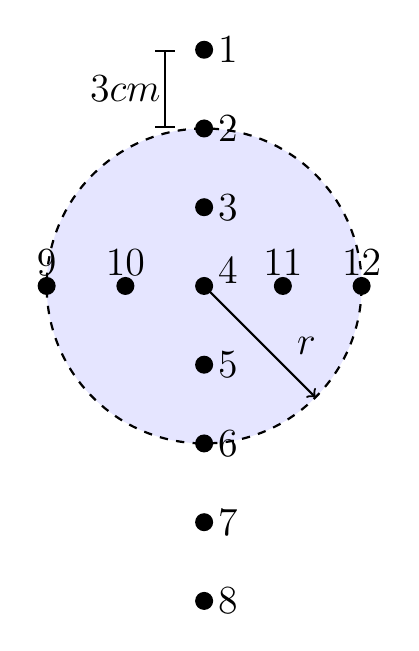
\begin{tikzpicture}[style={font=\Large}]
%\draw[thick,dashed] (0,0) circle (4cm);
\filldraw[fill=blue!10!white,thick,dashed] (0,0) circle (2cm);
\draw[|-|,thick] (-0.5,2) -- (-0.5, 3)node at (-1,2.5) {\textbf{$3cm$}};
\draw[->,thick] (0,0) -- (1.41421356, -1.41421356)node at (1.3,-1)[above] {\textbf{$r$}};
\draw[thick,fill] (0,3) circle (0.1cm) node at (0.3,3)[] {\textbf{$1$}};
\draw[thick,fill] (0,2) circle (0.1cm) node at (0.3,2)[] {\textbf{$2$}};
\draw[thick,fill] (0,1) circle (0.1cm) node at (0.3,1)[] {\textbf{$3$}};
\draw[thick,fill] (0,0) circle (0.1cm) node at (0.3,0.2)[] {\textbf{$4$}};
\draw[thick,fill] (0,-1) circle (0.1cm) node at (0.3,-1)[] {\textbf{$5$}};
\draw[thick,fill] (0,-2) circle (0.1cm) node at (0.3,-2)[] {\textbf{$6$}};
\draw[thick,fill] (0,-3) circle (0.1cm) node at (0.3,-3)[] {\textbf{$7$}};
\draw[thick,fill] (0,-4) circle (0.1cm) node at (0.3,-4)[] {\textbf{$8$}};
\draw[thick,fill] (-2,0) circle (0.1cm) node at (-2,0.3)[] {\textbf{$9$}};
\draw[thick,fill] (-1,0) circle (0.1cm) node at (-1,0.3)[] {\textbf{$10$}};
\draw[thick,fill] (1,0) circle (0.1cm) node at (1,0.3)[] {\textbf{$11$}};
\draw[thick,fill] (2,0) circle (0.1cm) node at (2,0.3)[] {\textbf{$12$}};
\end{tikzpicture}
\caption{Verwendeten Messplatte mit Umgebung des homogenen Magnetfeldes}
\label{fig:MessPlatte}
\end{figure}

Entsprechend Anweisung seitens unserer Betreuerin, als auch den Hinweisen der Aufgabenbeschreibung maßen wir den ersten und höchsten Ausschlag der Hallspannung für die jeweilige Spulenströme von $1 A$, $1.5 A$ und $2 A$ an den vorgegebenen Positionen der Messplatte (siehe Abbildung \ref{fig:MessPlatte}). Aufgrund der zuvor erwähnten  Empfindlichkeit der  Hallsonde führten wir die Messung für $1 A$ erneut durch, da diese anfangs uns falsch erschienen.


\newpage
 

\begin{table}
\begin{center}
\begin{tabular}{|c|c|c|c|}
\hline 
& I = 1 A & I = 1.5 A & I = 2 A \\ 
\hline 
Punkt & $U_h$ [mV] & $U_h$ [mV] & $U_h$ [mV] \\ 
\hline 
1 & 0.105 & 0.16 & 0.2 \\ 
\hline 
2 & 0.112 & 0.165 & 0.21 \\ 
\hline 
3 & 0.112 & 0.165 & 0.215 \\ 
\hline 
4 & 0.112 & 0.165 & 0.215 \\ 
\hline 
5 & 0.112 & 0.165 & 0.215 \\ 
\hline 
6 & 0.112 & 0.16 & 0.21 \\ 
\hline 
7 & 0.106 & 0.15 & 0.2 \\ 
\hline 
8 & 0.087 & 0.12 & 0.165 \\ 
\hline 
9 & 0.108 & 0.16 & 0.21 \\ 
\hline 
10 & 0.108 & 0.16 & 0.215 \\ 
\hline 
11 & 0.108 & 0.16 & 0.215 \\ 
\hline 
12 & 0.11 & 0.16 & 0.21 \\ 
\hline 
\end{tabular} 
\caption{Hallspannungen der Helmnholzspulenpaares}
\end{center}
\end{table}

\begin{center}                                       
  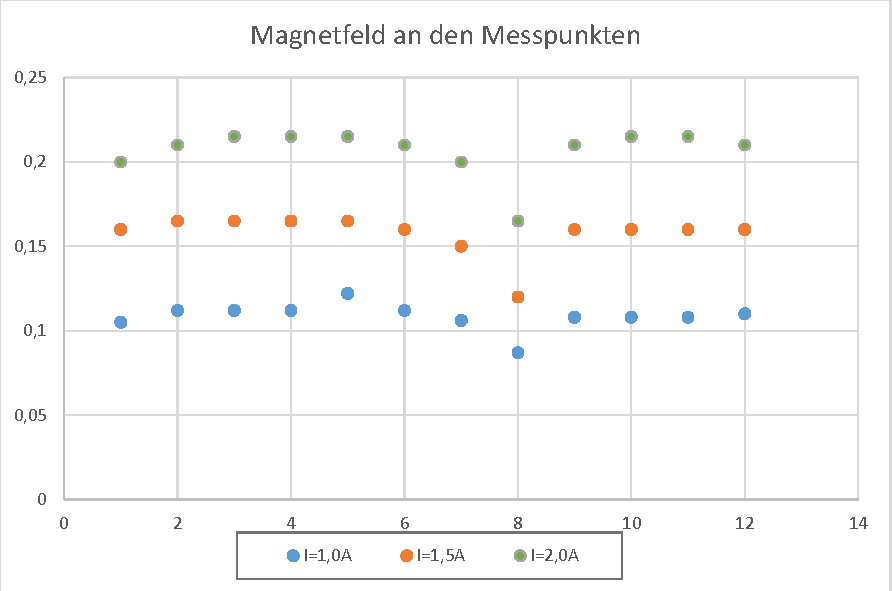
\includegraphics{./include/Bfeld.pdf} 
                          
\end{center} 

TABELLE MIT WERTEN IN ANHANGXXXXXX

Abbildung BFELD zeigt die magnetische Flussdichte abhängig von den Messpunkten. Zu sehen ist, dass das Feld im Radius von $6 cm$ um den Punkt 4 recht homogen ist. Dieser Aspekt lässt sich mit den Eigenschaften des Helmholtzspulenpaares bezüglich der Feldhomogenität vereinbaren. Außerdem ist ein deutlicher Abfall der magnetischen Flussdichte im Punkt 8 zu sehen, da dieser außerhalb der Radius liegt

\section{Kalibrieren der Hallsonde}
Um die Hallsonde möglichst genau zu Eichen wurde sie in die Mitte der Spule eingeführt und zehn Messungen der Hallspannung durchgeführt. Anhand der Formel für lange Spulen kann die magnetische Flussdichte der Spule bestimmt werden:
\begin{equation*}
B_{spule} = \mu_0 \cdot \frac{n \cdot I}{L}
\end{equation*}
Der Literaturwert für $\mu_0$ liegt bei $4\pi \cdot 10^{-7} \frac{N}{A^2}$.
%https://lp.uni-goettingen.de/get/text/4087
\newline
Die verwendete Spule hatte folgende Maßzahlen: L = 300mm, d = 20 mm, n = 750 Windungen.
\newline
Um die Eichgerade zu bestimmen wird das Gleichgewicht zwischen der Lorentzkraft und der elektrischen Kraft ausgenutzt:
\begin{eqnarray*}
F_{lorentz} &=& F_{elektrisch} \\
q \cdot v \cdot B_{spule} &=& q \cdot E \quad | \quad E = \frac{U_h}{d}\\
B_{spule} &=&\frac{1}{v \cdot d} \cdot U_h \Rightarrow m = \frac{1}{v \cdot d}
\end{eqnarray*}
Somit lässt sich ein linearer Zusammenhang zwischen Hallspannung und magnetischen Flussdichte herstellen. Die Steigung $m$ ist nur von der Spannung der Hallsonde abhängig und somit konstant. 
\newline
Sie lässt sich aus den Messwerten (siehe Tabelle \ref{tab:eichspule}) mit linearer Regression (siehe Abbildung BLABLABAL) berechnen und liegt bei $m = 0.146 \frac{s}{m^2}$. Außerdem stimmen die gemessenen Hallspannungen etwa mit den Messungen aus ref{•} überein.

\begin{minipage}[h]{0.35\linewidth}

\begin{tabular}{|c|c|c|}
\hline 
I [A] & $U_h$ [mV] & $B_{spule}$ [mT] \\ 
\hline 
0.199 & 0.094 & 0.625
 \\ 
\hline 
0.230 & 0.106 & 0.722
 \\ 
\hline 
0.287 & 0.135 & 0.901
 \\ 
\hline 
0.320 & 0.15 & 1.005
 \\ 
\hline 
0.363 & 0.17 & 1.140
 \\ 
\hline 
0.398 & 0.185 & 1.250
 \\ 
\hline 
0.445 & 0.205 & 1.398
 \\ 
\hline 
0.499 & 0.235 & 1.567
 \\ 
\hline 
0.540 & 0.25 & 1.696
 \\ 
\hline 
0.587 & 0.27 & 1.844
 \\ 
\hline 
\end{tabular} 
\captionof{table}{Berechnete magnetische Flussdichte der Eichspule}
\label{tab:eichspule}

\end{minipage}
\hfill
\begin{minipage}[h]{0.6\linewidth}

\begin{tikzpicture}[scale=0.9]
    \pgfplotsset{width=10cm,
        compat=1.10,
        legend style={font=\footnotesize}}
    \begin{axis}[
    xlabel={$B_{spule}$  [mT]},
    ylabel={$U_h$ [mV]},
    legend cell align=left,
    legend pos=north west]
    \addplot[only marks] table[row sep=\\]{
        X Y\\
 0.625   0.094\\
 0.722    0.106\\
 0.901   0.135\\
 1.005    0.15\\
 1.140   0.17\\
 1.250   0.185\\
 1.398    0.205\\
 1.567   0.235\\
 1.696    0.25\\
 1.844   0.27\\
    };
    \addlegendentry{Messpunkte}
    \addplot[no markers,red] table[row sep=\\,
    y={create col/linear regression={y=Y}}] % compute a linear regression from the
    %input table
    {
        X Y\\
 0.625   0.094\\
 0.722    0.106\\
 0.901   0.135\\
 1.005    0.15\\
 1.140   0.17\\
 1.250   0.185\\
 1.398    0.205\\
 1.567   0.235\\
 1.696    0.25\\
 1.844   0.27\\
    };
    \addlegendentry{%
        $\pgfmathprintnumber[precision=3]{\pgfplotstableregressiona} \cdot x
        \pgfmathprintnumber[print sign]{\pgfplotstableregressionb}$} %
    \end{axis}
\end{tikzpicture}
\captionof{figure}{Eichspulengerade}
\label{fig:Eichspulengerade}
\end{minipage}

	

    

\section{Vergleich zwischen gemessenen und berechneten Wert des Mittenfeldes zwischen den Helmholtzspulen}
Um die Genauigkeit unserer Messwerte und dem daraus berechneten Magnetfeld zu überprüfen haben wir für die drei Stromstärken $1 A$,$1.5 A$, und $2 A$ unseren gemessenen als auch den Soll-Wert vergleichen. Die Abweichungen vom Sollwert sind in Prozent angegeben.
 
 In XX sieht man, dass aufgrund der zuvor beschriebenen Messunsicherheiten seitens der Messgeräte (siehe Kapitel 1,111) sowie den sich fortpflanzenden Fehlern während der Nullabstimmung als auch der in 1.2 beschrieben Eichung, Abweichungen auftreten. So erhielten wir dennoch Abweichungen die noch sehr gering sind.
 
 Im Nachfolgenden wird nun mit dem Sollwert weiter gerechnet um die Fortpflanzung der zuvor beschrieben Messunsicherheiten zu vermeiden.
 
 
\section{Messung des Durchmessers der Elektronenkreisbahn im Fadenstrahlrohr}
\paragraph{In Abhängigkeit der Anodenspannung}
Entsprechend der Aufgabenbeschreibung bauten wir den Versuch auf und bestimmten für Anodenspannungen von 125V bis 250V bei jeweils 1A und 2A die zugehörigen Durchmesser der Elektronenkreisbahn. Hierfür wählten wir einen adjazenten Abstand von 25V. Parallaxenfehler bei der Bestimmung des Durchmessers wurden gemäß Anordnung möglichst klein gehalten. Jedoch stellte sich das exakte bestimmen des Durchmessers als dennoch schwierig heraus, was an dem stellenweise diffusen Elektronenstrahl zuzuschreiben ist. Um möglichst gute Ergebnisse zu erzielen überprüften wir jeweils die Bestimmung des Durchmessers des jeweils anderen. Aufgrund der zu großen Kreisbahn und demndamit überschrittenen Messbereich unserer Versuchsanordnung konnten wir bei 1A für Anodenspannungen größer als 200V keinen Durchmesser der Kreisbahn bestimmen. Hingegen konnten wir bei 2A für alle Anodenspannungen einen Durchmesser bestimmen. So ermittelten wir die in Abbildung XX gezeigten Messwerte. 




\paragraph{In Abhängigkeit des Spulenstroms}
Nun untersuchten wir entsprechend der Aufgabenbeschreibung in b die  Durchmesser der Elektronenkreisbahn für zwei feste Beschleunigungsspannungen (150V und 250V) für Spulenströme zwischen 1A bis 2A. Hierfür wählten den adjazenten Abstand von 0.2A. Auch hier trat das soeben beschriebene Problem des Diffusen Elektronenstrahls auf. Bis auf den Messwert für 1A bei 250V konnten wir für jede Konfiguration einen Durchmesser bestimmen, welche in Abbildung XX zu sehen sind.






